\documentclass[12pt]{article}
\usepackage{amsthm,amssymb,amsmath,amsfonts}
\usepackage[a4paper, top=25mm, bottom=30mm, left=25mm, right=25mm]{geometry}
\usepackage[pagebackref=false,colorlinks,linkcolor=black,citecolor=black]{hyperref}
\usepackage[nameinlink]{cleveref}
 \AtBeginDocument{%
    \crefname{equation}{برابری}{equations}%
    \crefname{chapter}{فصل}{chapters}%
    \crefname{section}{بخش}{sections}%
    \crefname{appendix}{پیوست}{appendices}%
    \crefname{enumi}{مورد}{items}%
    \crefname{footnote}{زیرنویس}{footnotes}%
    \crefname{figure}{شکل}{figures}%
    \crefname{table}{جدول}{tables}%
    \crefname{theorem}{قضیه}{theorems}%
    \crefname{lemma}{لم}{lemmas}%
    \crefname{corollary}{نتیجه}{corollaries}%
    \crefname{proposition}{گزاره}{propositions}%
    \crefname{definition}{تعریف}{definitions}%
    \crefname{result}{نتیجه}{results}%
    \crefname{example}{مثال}{examples}%
    \crefname{remark}{نکته}{remarks}%
    \crefname{note}{یادداشت}{notes}%
    \crefname{observation}{مشاهده}{observations}%
    \crefname{algorithm}{الگوریتم}{algorithms}%
    \crefname{cproof}{برهان}{cproofs}%
}

\usepackage{tikz}
\usepackage{graphicx}
\usepackage{booktabs}
\usepackage{color}
\usepackage{graphicx}
\usepackage{subcaption}

\usepackage{setspace}
\doublespacing

\usepackage{titletoc}
\usepackage{tocloft}
\usepackage{enumitem}
\usepackage{amsmath, amssymb}
\usepackage{algorithm}
\usepackage[noend]{algorithmic}
\renewcommand{\algorithmicrequire}{\textbf{Input:}}
\renewcommand{\algorithmicensure}{\textbf{Output:}}

\usepackage{tabularx}
\makeatletter
\newcommand{\multiline}[1]{%
  \begin{tabularx}{\dimexpr\linewidth-\ALG@thistlm}[t]{@{}X@{}}
    #1
  \end{tabularx}
}
\makeatother

\usepackage{float}
\usepackage{verbatim}
\makeindex
\usepackage{sectsty}
\usepackage{xepersian}
\SepMark{-}
\settextfont[Scale=1.2,Path=fonts/,BoldFont=B Nazanin Bold.ttf]{B Nazanin.ttf}
\setlatintextfont{Times New Roman}
\renewcommand{\labelitemi}{$\bullet$}

\theoremstyle{definition}
\newtheorem{definition}{تعریف}[section]
\newtheorem{remark}[definition]{نکته}
\newtheorem{note}[definition]{یادداشت}
\newtheorem{example}[definition]{نمونه}
\newtheorem{question}[definition]{سوال}
\newtheorem{remember}[definition]{یاداوری}
\newtheorem{observation}[definition]{مشاهده}
\theoremstyle{theorem}
\newtheorem{theorem}[definition]{قضیه}
\newtheorem{lemma}[definition]{لم}
\newtheorem{proposition}[definition]{گزاره}
\newtheorem{corollary}[definition]{نتیجه}
\newtheorem*{cproof}{برهان}




\begin{document}
\fontsize{12pt}{14pt}\selectfont

\begin{minipage}{0.1\textwidth}

\includegraphics[width=3cm]{etc/IUST}
\end{minipage}%
\hfill%
\begin{minipage}{0.6\textwidth}\centering
\fontsize{13pt}{13pt}\selectfont
به‌ نام خدا \\
\textbf{درس یادگیری عمیق} \\
\textbf{تمرین سری ششم}\\
استاد درس : دکتر محمدرضا محمدی \\
دستیاران :  مهدی خورشا، سید محمد موسوی،\\ امیرحسین نمازی
\\
\vspace{0.25cm}
\begingroup
\fontsize{11pt}{11pt}\selectfont
دانشگاه علم و صنعت ایران، دانشکده مهندسی کامپیوتر \\
نیمسال دوم تحصیلی 1403 - 1404 \\
\endgroup
\end{minipage}%
\hfill%
\begin{minipage}{0.1\textwidth}

\end{minipage}

\vspace{0.5cm}

\noindent\rule{\textwidth}{1pt}

\centering {\fontsize{18}{22}\selectfont \textbf{مهلت تحویل : 1404/02/23 }}\\
{\fontsize{14}{22}\selectfont \textbf{لطفا به نکات موجود در سند قوانین انجام و تحویل تمرین ها دقت فرمایید. }}

\begin{enumerate}

    \section*{سوالات تئوری}
    \item 
\includegraphics[width=1cm]{figs/Forbidden_AI.jpg}
    بر اساس \href{https://arxiv.org/abs/2309.06180}{ مقاله} لطفا به سوالات زیر پاسخ دهید (۱۰ نمره):
    \begin{enumerate}
        \item چالش‌های اصلی در زمینه مدیریت حافظه که سیستم‌های خدمات‌دهی \lr{LLM} موجود مواجه هستند، چیست؟
        \item  \lr{PagedAttention} چگونه به این چالش‌ها پاسخ می‌دهد؟ 
        \item اهمیت اشتراک‌گذاری حافظه کش \lr{KV} در سیستم‌های خدمات‌دهی \lr{LLM} را مورد بحث قرار دهید. \lr{vLLM} چگونه اشتراک‌گذاری حافظه را تسهیل می‌کند و این موضوع چه پیامدهایی برای توان عملیاتی کلی سیستم دارد؟ پاسخ خود را با جزئیات موجود در مقاله بیان کنید.
    \end{enumerate}
     
    
    
    \href{https://www.youtube.com/watch?v=5ZlavKF_98U}{ویدیوی ارائه نویسندگان مقاله در یک کنفرانس}

    \item 
\includegraphics[width=1cm]{figs/Forbidden_AI.jpg}
    	با توجه به \lr{Multi-Head Attention} به پرسش‌های زیر پاسخ دهید (10 نمره):
        \begin{enumerate}
            \item	چرا در مدل‌های ترنسفورمر از توجه چندسری (\lr{Multi-Head Attention}) استفاده می‌شود؟ و این سرهای توجه چه نوع اطلاعاتی را می‌توانند یاد بگیرند؟
            \item 	فرض کنید یک مدل آموزش‌دیده داریم که بر پایه‌ی توجه چندسری (\lr{Multi-Head Attention}) ساخته شده است و می‌خواهیم برای افزایش سرعت پیش‌بینی، سرهای توجه کم‌اهمیت‌تر را حذف (\lr{Prune}) کنیم. چگونه می‌توانیم آزمایش‌هایی طراحی کنیم تا اهمیت هر سر توجه را اندازه‌گیری کنیم؟
            \item 	حذف سرهای توجه چه اثری روی وظایف پایین‌دستی (مثل طبقه‌بندی یا ترجمه) دارد؟ از چه معیارهایی برای ارزیابی تأثیر حذف سرها استفاده کنیم؟
            \item 	آیا می‌توان از یادگیری تقویتی (\lr{Reinforcement Learning}) برای انتخاب دینامیک سرهای توجه استفاده کرد؟
        \end{enumerate}
        (اختیاری: می‌توانید از \href{https://arxiv.org/abs/1905.10650}{مقاله}  بهره بگیرید.)
    \item 
\includegraphics[width=1cm]{figs/Forbidden_AI.jpg}
    در رابطه با \lr{Additive Attention} به پرسش‌های زیر پاسخ دهید (۱۰ نمره):
    \begin{enumerate}
        \item آیا ایده‌ی خوبی است که در مدل ترنسفورمر، توجه ضرب نقطه‌ای مقیاس‌شده (\lr{Scaled Dot-Product Attention}) را با توجه جمعی (\lr{Additive Attention}) جایگزین کنیم؟ چرا؟
        \item آیا می‌توان ترکیبی از این دو نوع توجه استفاده کرد؟
        \item یک توجه چند سر \lr{additive} با ۳ سر را در نظر بگیرید. ابعاد \lr{query} ،\lr{key} و \lr{value} را به ترتیب ۱۰، ۲۰، ۳۰ در نظر بگیرید فرض کنید هر کدام از سرها به ابعاد ۱۰۰ تبدیل شوند. همچنین در نظر داشته باشید که خروجی نهایی ۵۰ میباشد. با فرض اینکه دنباله ورودی ۶۴ تایی باشد، تعداد پارامترها را مشخص کنید.
    \end{enumerate}

    \item 
\includegraphics[width=1cm]{figs/Forbidden_AI.jpg}
    در رابطه با کاربرد مدل‌های \lr{transformer} در سری‌های زمانی به سوالات زیر پاسخ دهید (۲۰ نمره):
    \begin{enumerate}
        \item چه زمانی استفاده از ترنسفورمر در سری زمانی مناسب‌تر از استفاده از \lr{LSTM} است؟
        \item چگونه داده‌های سری زمانی باید برای ورودی به ترنسفورمر پیش‌پردازش شوند؟
        \item چه تفاوتی بین ترنسفورمر استاندارد و ترنسفورمر مخصوص سری زمانی (مانند \lr{Time Series Transformer}  یا \lr{Informer}) وجود دارد؟
        \item چگونه می‌توان از ترنسفورمر برای پیش‌بینی چند مرحله‌ای (\lr{multi-step forecasting}) در سری‌های زمانی استفاده کرد؟
        \item نحوه‌ی عملکرد مدل \lr{iTransformer} جهت وظیفه‌ی \lr{Time Series Forecasting} را توضیح دهید. (میتوانید از \href{https://arxiv.org/pdf/2310.06625}{مقاله} بهره بجویید.)
    \end{enumerate}
    
    	
    \section*{سوالات عملی} 
    \item 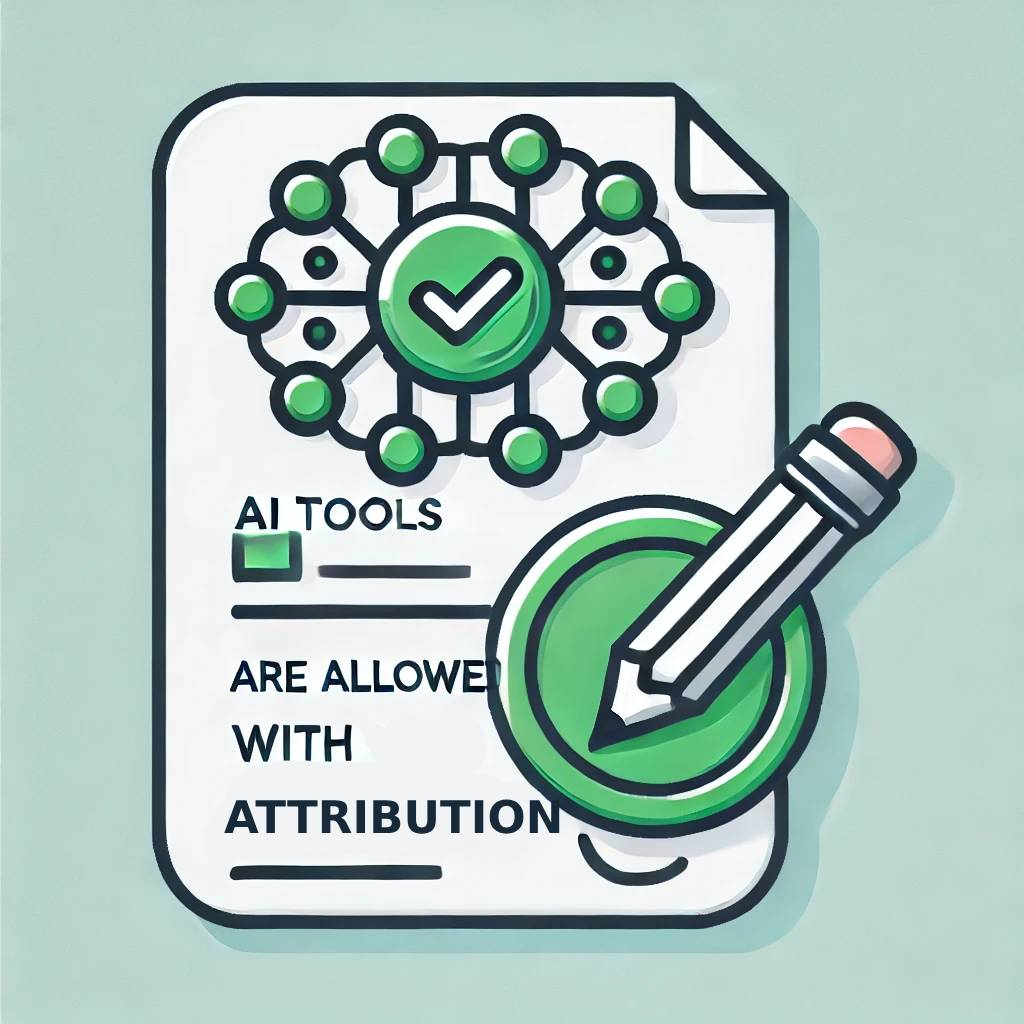
\includegraphics[width=1cm]{figs/Allowed_with_contributino.jpg}
    در این تمرین با مدل \lr{ViT} برای دسته‌بندی تصاویر آشنا خواهید شد. شما یک مدل \lr{pretrained}  را با استفاده از \lr{Hugging Face} بارگذاری می‌کنید، وزن‌های \lr{attention} آن را تجزیه و تحلیل می‌کنید و برای درک بهتر مکانیزم توجه و رفتار آن در مدل پیش آموخته شده، وزن‌های یادگیری شده را نمایش خواهید داد. در بخش بعدی آن را روی دیتاست \lr{CIFAR-10}  آموزش خواهید داد ( \lr{fine-tune}) و در نهایت نقش \lr{attention head}ها را بررسی می‌کنید. در این سوال از نوتبوک \lr{Q5.ipynb} استفاده کنید.(۲۵ نمره)
    \begin{enumerate}
        \item از کتابخانه \lr{transformers} در \lr{Hugging Face} برای بارگذاری مدل \lr{pretrained} استفاده کنید (ترجیحا مدل \lr{google/vit-base-patch16-224}). در این بخش پس از انجام پیش‌پردازش تصویر مورد نظر، با استفاده از مدل پیش‌آموزش دیده خروجی مدل را بدست آورده و ۵ کلاس برتر پیش‌بینی شده را  همراه با احتمالات پیش‌بینی محاسبه کنید. 
        \item با فراخوانی مدل می‌توانید به وزن‌های مکانیزم توجه برای تصویر مورد‌نظر دسترسی داشته باشید. در این بخش \lr{attention weights} مربوط به توکن [\lr{CLS}] را استخراج کنید و نقشه‌های توجه این توکن را برای تمام لایه و \lr{head}ها به صورت جداگانه نمایش دهید.
        \item \href{https://aclanthology.org/2020.acl-main.385.pdf}{\lr{Attention Rollout}} روشی برای مصورسازی و تفسیر مکانیزم توجه در مدل‌های \lr{Transformer} است. در این روش با ضرب تجمعی ماتریس‌های \lr{attention} در لایه‌ها، مسیر توجه از ورودی تا خروجی مدل به‌صورت یکپارچه نمایش داده می‌شود. با استفاده از روش \lr{attention rollout} و توضیحات داخل نوتبوک جریان تاثیر هر \lr{patch} از تصویر روی توکن \lr{cls} را در طول لایه‌ها نمایش دهید. 
        \item مدل پیش‌آموخته شده را بر روی دیتاست \lr{CIFAR-10} آموزش (\lr{fine-tune}) دهید و دقت آن را گزارش کنید. 
        \item در این بخش پس از آموزش روی دادگان بررسی کنید که دور ریختن یک یا چند \lr{head} چه تاثیری در عملکرد مدل ایجاد می‌کند. با استفاده از داده \lr{validation} تحلیل کنید کدام \lr{head}ها نقش مهمتری در تصمیم‌گیری مدل دارند.  
    \end{enumerate}
    \item 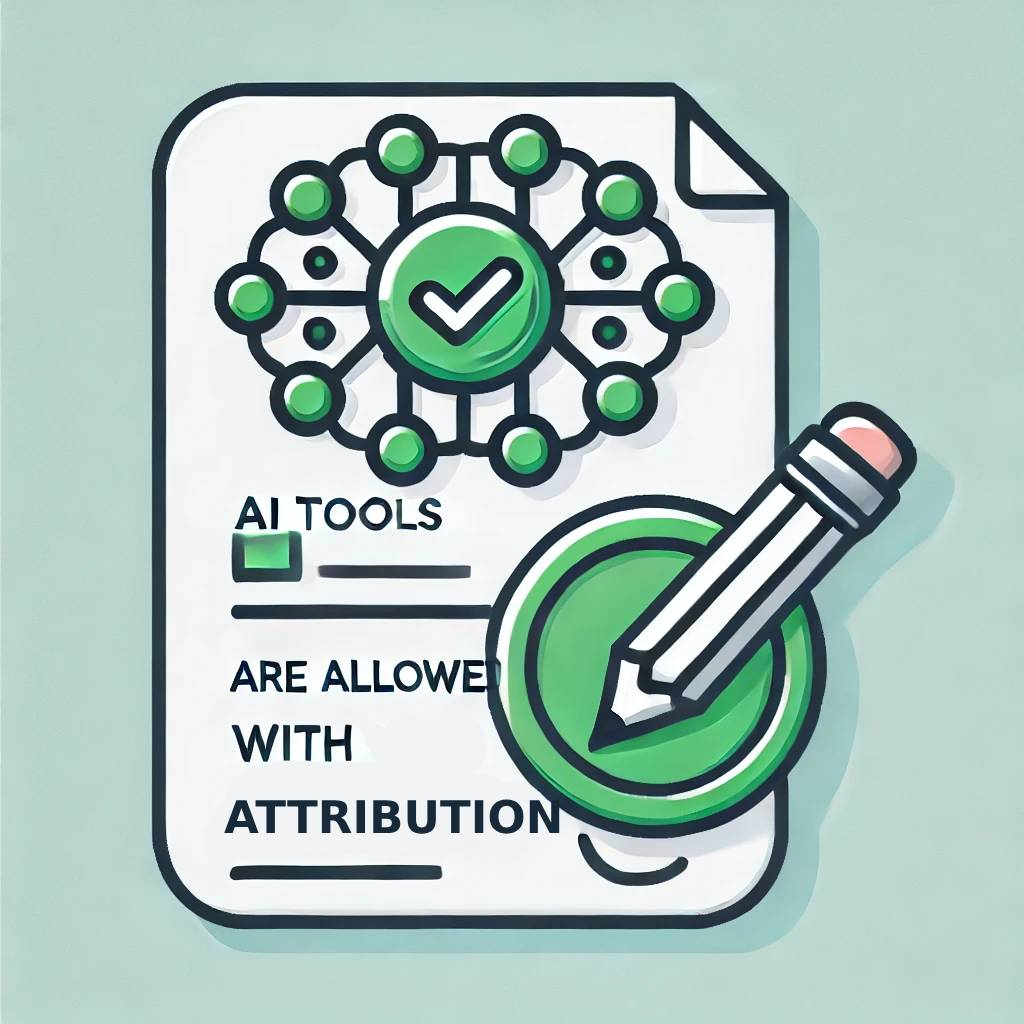
\includegraphics[width=1cm]{figs/Allowed_with_contributino.jpg}
    در این تمرین، مدل ترجمه ماشینی مبتنی بر توجهی را آموزش خواهید داد تا کلمات را از انگلیسی به \lr{Pig-Latin}    ترجمه کنید.\lr{Pig-Latin}یک بازی زبانی است که در آن قوانین به صورت مستقل برای هر کلمه اعمال می    شود:    (۲۵ نمره)
    \begin{itemize}
        \item اگر اولین حرف یک کلمه، حرف بی صدای انگلیسی باشد، آن حرف به انتهای کلمه منتقل شده و حروف \lr{\lr{ay}}به انتهای کلمه اضافه می  شوند: \lr{team → eamtay} .
        \item  اگر اولین حرف، یک حرف صدادار انگلیسی باشد، کلمه بدون تغییر باقی می ماند و حروف \lr{way } به انتهای کلمه اضافه می شوند: \lr{impress → impressway}.
        \item برخی از جفت حروف مانند \lr{sh} به عنوان یک بلوک در نظر گرفته  میشوند و به صورت کل به انتهای رشته منتقل میشوند:
        \lr{shopping → oppingshay}
    \end{itemize}
    هدف این است که مدل ترجمه ماشینی قوانین را به طور ضمنی از طریق جفت های کلمات (\lr{English}, \lr{Pig-Latin}) که \lr{source}  کلمه انگلیسی و \lr{target} ترجمه آن به  \lr{Pig-Latin} است، یاد بگیرد.\\
    داده ها:\\
    در این تمرین از دو مجموعه داده استفاده خواهید کرد:\\
    \begin{itemize}
    \item واژگان مجموعه داده کوچک شامل ۲۹ نشانه است: ۲۶ حرف استاندارد الفبا (همه با حروف کوچک)، نماد خط تیره “-” و دو نشانه \lr{<SOS>} و \lr{<EOS>} که به ترتیب شروع و پایان یک دنباله را نشان می‌دهند. مجموعه داده شامل ۳۱۹۸ جفت (\lr{English}, \lr{Pig-Latin}) منحصر به فرد است.
    \item مجموعه داده بزرگ‌تر، شامل 2۰,۰۰۰ کلمه انگلیسی پرکاربردتر است که با مجموعه داده قبلی ترکیب می‌شود و 22402 کلمه منحصر به فرد به دست می‌آید
    \end{itemize}
    \begin{enumerate}
    \item به بخش \lr{scaled dot product attention} در نوتبوک \lr{pigLatin} مراجعه کرده و بخش‌های مشخص‌شده را تکمیل کنید.
    \item مدل \lr{Transformer} را با استفاده از \lr{hidden size}  های 32 و 64 و با استفاده از مجموعه داده کوچک و بزرگ (در مجموع ۴ اجرا) اجرا کنید و اثرات افزایش ظرفیت مدل از طریق \lr{hidden size} و افزایش اندازه مجموعه داده را گزارش کنید.
    \item به معماری \lr{Transformer} در شکل زیر نگاه کنید. در هر لایه ابتدا \lr{CausalScaledDotAttention} را به ورودی‌های \lr{decoder} و سپس \lr{ScaledDotAttention} را به \lr{encoder annotations} اعمال می‌کنیم. \lr{\_\_init\_\_} بخش \lr{decoder} را طوری تغییر دهید که فقط از \lr{ScaledDotAttention} استفاده کند. نتایج خود را حالت قبلی مقایسه کنید.
    \end{enumerate}
    \begin{figure}[h]  
            \centering
            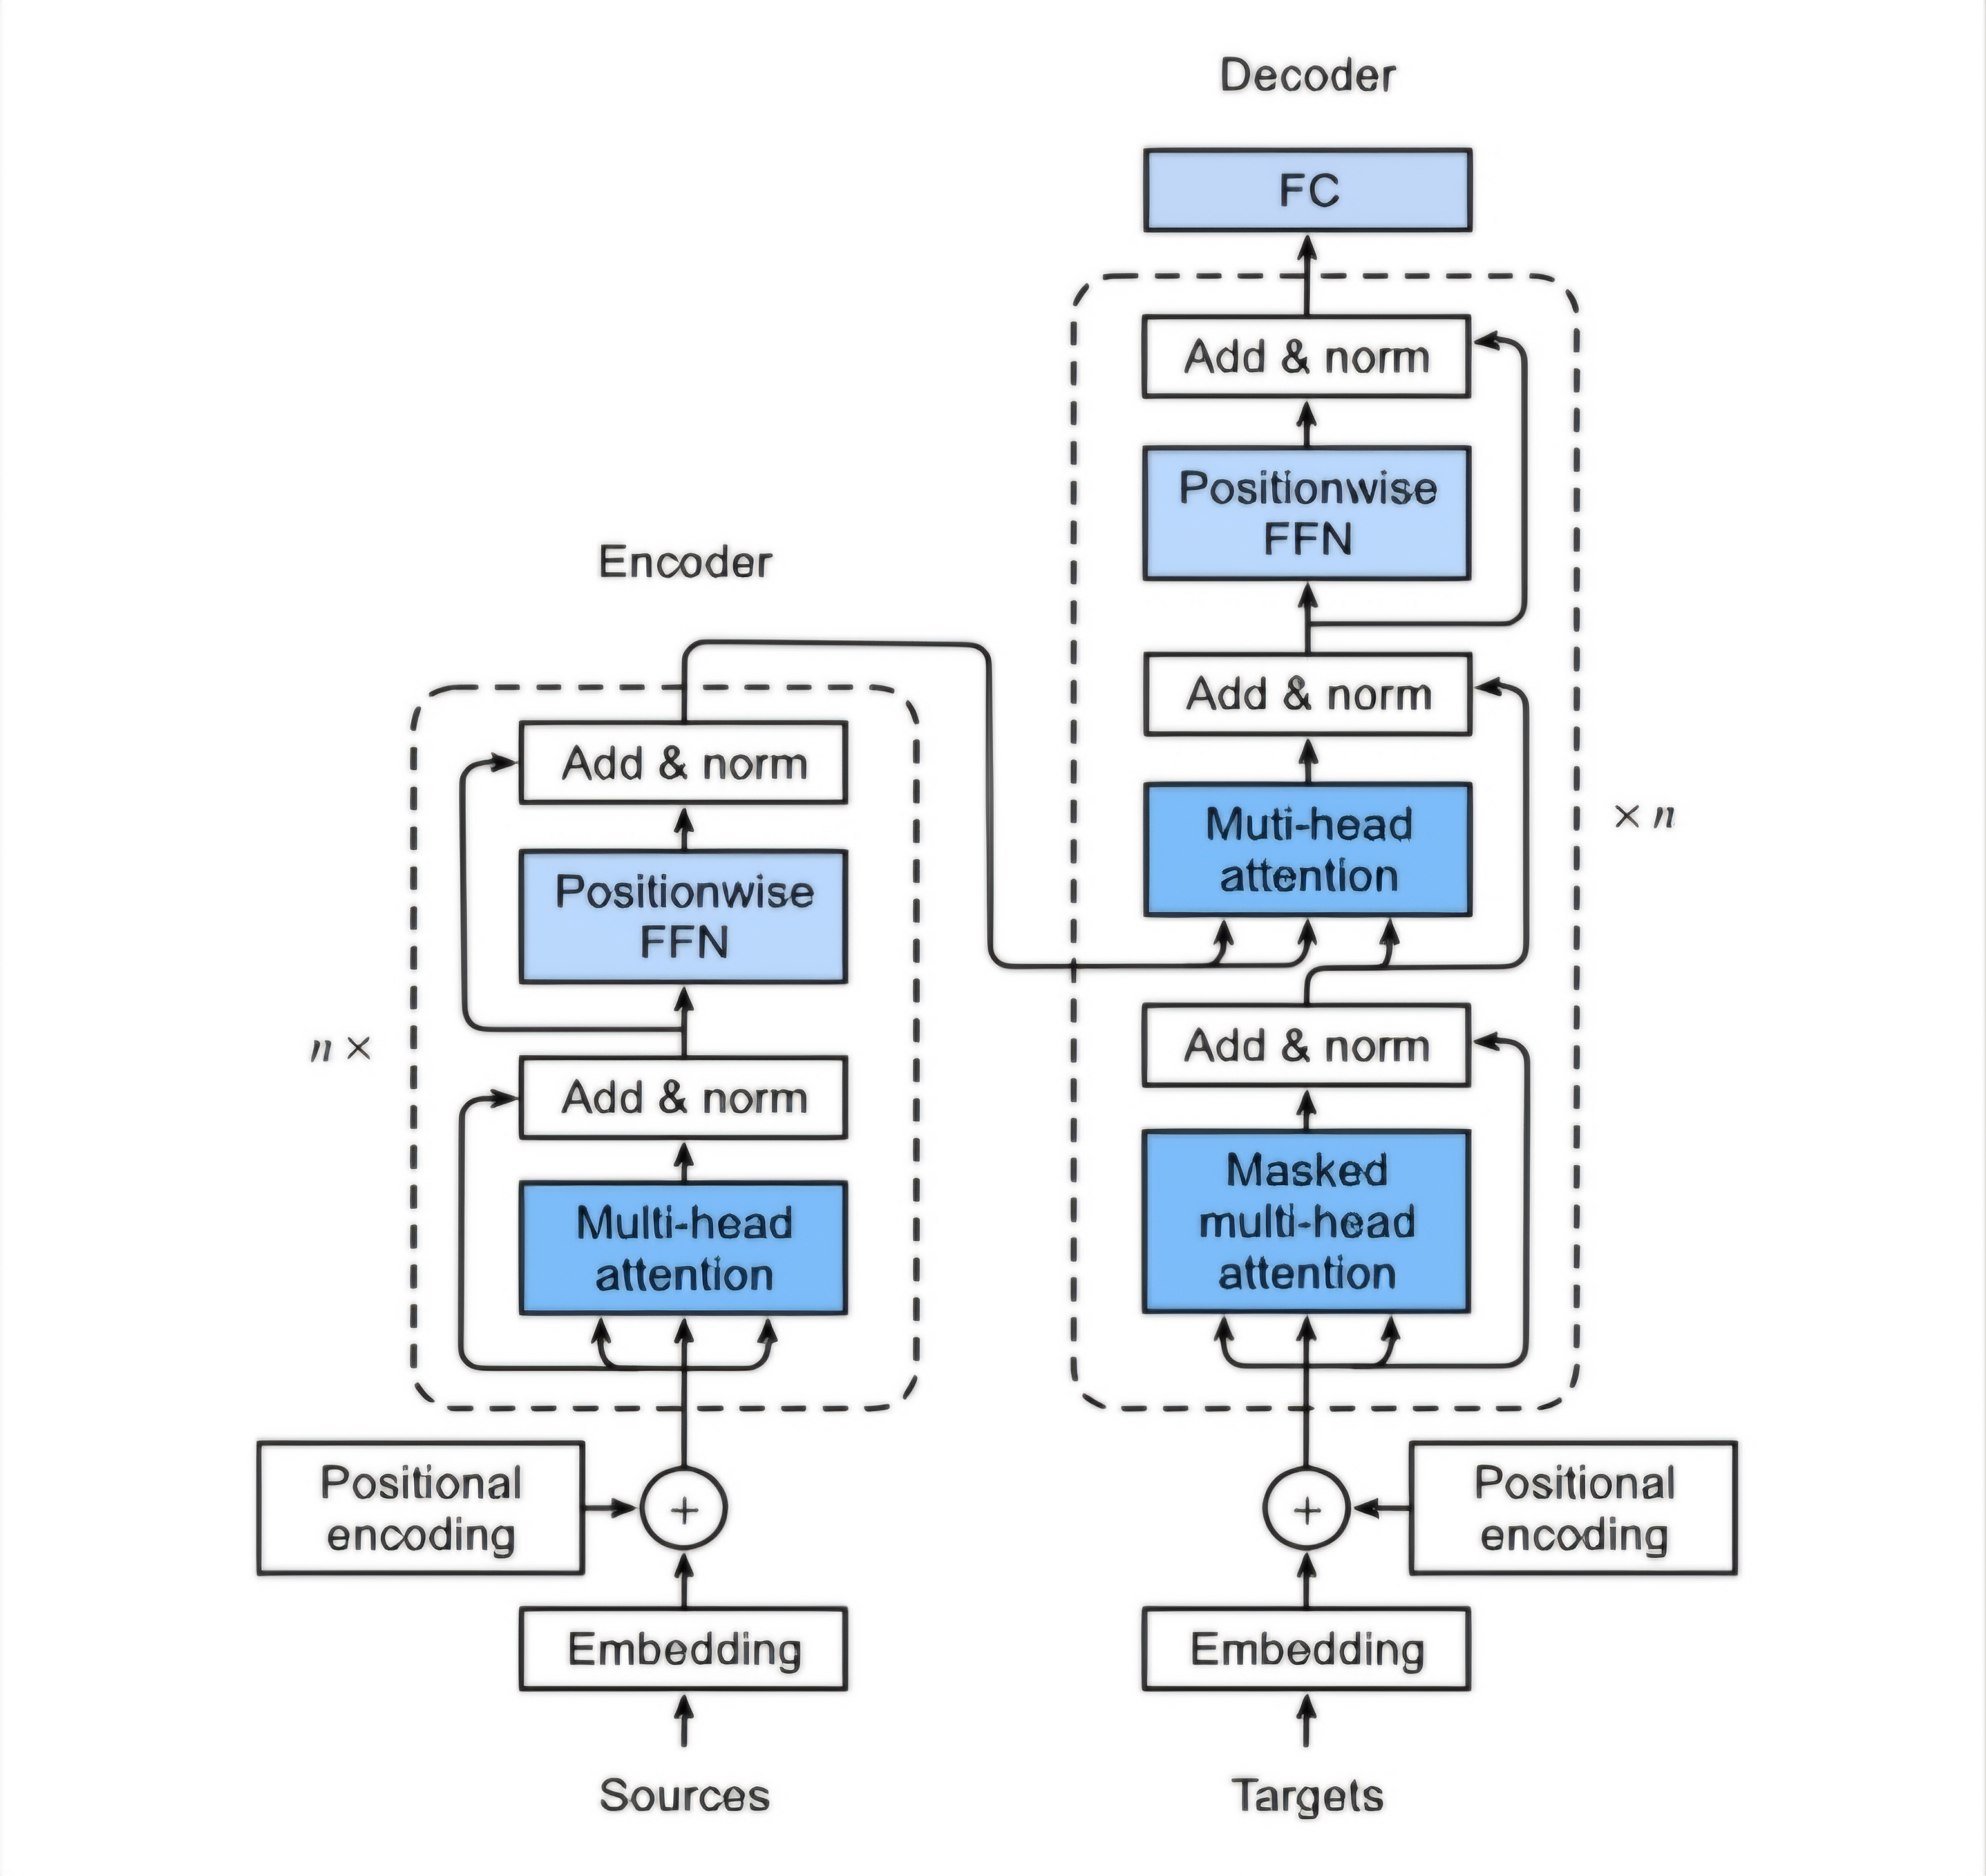
\includegraphics[width=\textwidth]{figs/Q6.jpg}
            \label{fig:num_pic}  
        \end{figure}
    

\end{enumerate}



\end{document}


